\documentclass[tikz,border=5pt]{standalone}
\usepackage{ctex,amsmath}
\usetikzlibrary{arrows.meta,calc}
\tikzset{>=Latex,copper/.style={orange!70!black},wire/.style={blue!65!black,thick}}
\newcommand{\resistorH}[3]{\draw[wire](#1,#2)--++(.2,0) ++(0,-.13)rectangle++(.65,.26);\draw[wire](#1+.85,#2)--++(.2,0);\node[above]at(#1+.525,#2+.18){$#3$};}
\newcommand{\coil}[3]{
  \draw[wire](#1,.8)--(#1,1.0);
  \draw[wire] (#1,1.0)arc[start angle=-90,end angle=90,radius=.2]
  arc[start angle=-90,end angle=90,radius=.2]
  arc[start angle=-90,end angle=90,radius=.2]
  arc[start angle=-90,end angle=90,radius=.2];
  \draw[wire](#1,2.6)--(#1,2.8);
  \draw[wire,fill=white](#1,2.8)circle[radius=.045](#1,.8)circle[radius=.045];
  \fill(#1-.13,2.48)circle[radius=.04];
  \node[above left]at(#1-.12,2.85){$a_{#2}$};\node[below left]at(#1-.12,.65){$b_{#2}$};
  \node[left]at(#1-.14,1.7){$N_{#2}$};
}
\begin{document}
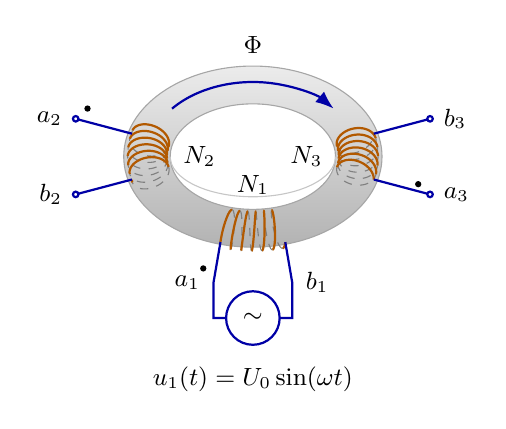
\begin{tikzpicture}[font=\small]
\shade[even odd rule,top color=gray!15,bottom color=gray!60]
 (0,0)ellipse[x radius=1.64,y radius=1.15]
 (0,0)ellipse[x radius=1.05,y radius=.67];
\draw[gray!70](0,0)ellipse[x radius=1.64,y radius=1.15];
\draw[gray!70](0,0)ellipse[x radius=1.05,y radius=.67];
\draw[gray!45](-1.05,0)arc[start angle=180,end angle=360,x radius=1.05,y radius=.51];
\newcommand{\corebackwires}{
\draw[gray,dashed,thin] plot coordinates {(-0.261981,-0.676456) (-0.259893,-0.677254) (-0.257878,-0.678430) (-0.255937,-0.679982) (-0.254073,-0.681907) (-0.252286,-0.684204) (-0.250578,-0.686868) (-0.248951,-0.689897) (-0.247404,-0.693285) (-0.245940,-0.697027) (-0.244558,-0.701119) (-0.243261,-0.705553) (-0.242047,-0.710324) (-0.240917,-0.715424) (-0.239873,-0.720846) (-0.238913,-0.726581) (-0.238038,-0.732621) (-0.237247,-0.738956) (-0.236541,-0.745578) (-0.235919,-0.752477) (-0.235380,-0.759641) (-0.234924,-0.767060) (-0.234550,-0.774723) (-0.234257,-0.782619) (-0.234043,-0.790734) (-0.233908,-0.799058) (-0.233851,-0.807578) (-0.233870,-0.816279) (-0.233963,-0.825151) (-0.234129,-0.834178) (-0.234366,-0.843347) (-0.234673,-0.852645) (-0.235046,-0.862057) (-0.235485,-0.871569) (-0.235988,-0.881166) (-0.236551,-0.890834) (-0.237172,-0.900558) (-0.237850,-0.910324) (-0.238582,-0.920116) (-0.239365,-0.929920) (-0.240196,-0.939721) (-0.241074,-0.949503) (-0.241994,-0.959253) (-0.242956,-0.968954) (-0.243954,-0.978593) (-0.244988,-0.988154) (-0.246053,-0.997624) (-0.247147,-1.006987) (-0.248267,-1.016230) (-0.249409,-1.025338) (-0.250572,-1.034298) (-0.251751,-1.043096) (-0.252944,-1.051718) (-0.254148,-1.060151) (-0.255359,-1.068383) (-0.256574,-1.076401) (-0.257791,-1.084192) (-0.259007,-1.091746) (-0.260218,-1.099050) (-0.261421,-1.106093) (-0.262614,-1.112865) (-0.263793,-1.119356) (-0.264956,-1.125555) (-0.266099,-1.131452) (-0.267221,-1.137040) (-0.268317,-1.142310) (-0.269386,-1.147253) (-0.270425,-1.151862) (-0.271431,-1.156131) (-0.272401,-1.160052) (-0.273334,-1.163620) (-0.274227,-1.166829) (-0.275077,-1.169675) (-0.275883,-1.172154) (-0.276641,-1.174261) (-0.277351,-1.175993) (-0.278010,-1.177348) (-0.278616,-1.178324) (-0.279168,-1.178920) (-0.279664,-1.179135) (-0.280101,-1.178968)};
\draw[gray,dashed,thin] plot coordinates {(-0.162816,-0.689571) (-0.161277,-0.690257) (-0.159786,-0.691324) (-0.158344,-0.692772) (-0.156951,-0.694597) (-0.155608,-0.696797) (-0.154317,-0.699369) (-0.153077,-0.702309) (-0.151889,-0.705612) (-0.150752,-0.709274) (-0.149669,-0.713290) (-0.148638,-0.717652) (-0.147659,-0.722355) (-0.146733,-0.727392) (-0.145860,-0.732754) (-0.145039,-0.738434) (-0.144271,-0.744424) (-0.143554,-0.750713) (-0.142888,-0.757292) (-0.142274,-0.764153) (-0.141709,-0.771283) (-0.141194,-0.778672) (-0.140728,-0.786309) (-0.140311,-0.794183) (-0.139940,-0.802280) (-0.139615,-0.810590) (-0.139336,-0.819099) (-0.139101,-0.827794) (-0.138909,-0.836662) (-0.138758,-0.845690) (-0.138648,-0.854863) (-0.138577,-0.864168) (-0.138544,-0.873591) (-0.138547,-0.883116) (-0.138585,-0.892730) (-0.138656,-0.902418) (-0.138759,-0.912164) (-0.138892,-0.921955) (-0.139054,-0.931775) (-0.139242,-0.941609) (-0.139455,-0.951442) (-0.139692,-0.961259) (-0.139950,-0.971044) (-0.140228,-0.980784) (-0.140524,-0.990463) (-0.140837,-1.000066) (-0.141163,-1.009579) (-0.141502,-1.018986) (-0.141852,-1.028274) (-0.142211,-1.037429) (-0.142576,-1.046436) (-0.142947,-1.055281) (-0.143321,-1.063951) (-0.143696,-1.072434) (-0.144072,-1.080714) (-0.144445,-1.088781) (-0.144814,-1.096622) (-0.145178,-1.104224) (-0.145534,-1.111577) (-0.145882,-1.118668) (-0.146218,-1.125487) (-0.146543,-1.132024) (-0.146853,-1.138268) (-0.147148,-1.144211) (-0.147426,-1.149842) (-0.147685,-1.155153) (-0.147925,-1.160137) (-0.148143,-1.164785) (-0.148339,-1.169090) (-0.148511,-1.173047) (-0.148658,-1.176648) (-0.148778,-1.179889) (-0.148871,-1.182764) (-0.148935,-1.185269) (-0.148970,-1.187401) (-0.148974,-1.189155) (-0.148947,-1.190530) (-0.148888,-1.191523) (-0.148796,-1.192133) (-0.148670,-1.192359) (-0.148510,-1.192200)};
\draw[gray,dashed,thin] plot coordinates {(-0.062412,-0.696524) (-0.061434,-0.697133) (-0.060478,-0.698124) (-0.059545,-0.699498) (-0.058635,-0.701252) (-0.057747,-0.703384) (-0.056881,-0.705889) (-0.056038,-0.708765) (-0.055217,-0.712006) (-0.054418,-0.715609) (-0.053640,-0.719567) (-0.052883,-0.723874) (-0.052148,-0.728524) (-0.051432,-0.733510) (-0.050737,-0.738824) (-0.050062,-0.744458) (-0.049405,-0.750403) (-0.048767,-0.756650) (-0.048148,-0.763190) (-0.047545,-0.770013) (-0.046959,-0.777107) (-0.046390,-0.784463) (-0.045836,-0.792069) (-0.045297,-0.799913) (-0.044772,-0.807983) (-0.044260,-0.816267) (-0.043761,-0.824752) (-0.043274,-0.833425) (-0.042797,-0.842272) (-0.042331,-0.851281) (-0.041875,-0.860437) (-0.041427,-0.869726) (-0.040987,-0.879133) (-0.040555,-0.888646) (-0.040128,-0.898247) (-0.039707,-0.907924) (-0.039290,-0.917661) (-0.038877,-0.927443) (-0.038467,-0.937256) (-0.038060,-0.947083) (-0.037653,-0.956910) (-0.037247,-0.966721) (-0.036841,-0.976502) (-0.036434,-0.986238) (-0.036025,-0.995914) (-0.035614,-1.005514) (-0.035199,-1.015023) (-0.034781,-1.024429) (-0.034358,-1.033714) (-0.033930,-1.042867) (-0.033495,-1.051872) (-0.033055,-1.060715) (-0.032607,-1.069383) (-0.032152,-1.077863) (-0.031688,-1.086141) (-0.031216,-1.094205) (-0.030735,-1.102042) (-0.030244,-1.109640) (-0.029743,-1.116988) (-0.029232,-1.124074) (-0.028710,-1.130888) (-0.028177,-1.137418) (-0.027633,-1.143655) (-0.027077,-1.149589) (-0.026509,-1.155212) (-0.025930,-1.160513) (-0.025338,-1.165486) (-0.024734,-1.170122) (-0.024118,-1.174415) (-0.023490,-1.178357) (-0.022849,-1.181943) (-0.022196,-1.185167) (-0.021531,-1.188025) (-0.020854,-1.190511) (-0.020165,-1.192622) (-0.019464,-1.194355) (-0.018751,-1.195707) (-0.018027,-1.196676) (-0.017291,-1.197260) (-0.016545,-1.197459) (-0.015788,-1.197272)};
\draw[gray,dashed,thin] plot coordinates {(0.038467,-0.697263) (0.038877,-0.697829) (0.039290,-0.698779) (0.039707,-0.700111) (0.040128,-0.701824) (0.040555,-0.703914) (0.040987,-0.706380) (0.041427,-0.709216) (0.041875,-0.712418) (0.042331,-0.715982) (0.042797,-0.719901) (0.043274,-0.724171) (0.043761,-0.728783) (0.044260,-0.733731) (0.044772,-0.739008) (0.045297,-0.744605) (0.045836,-0.750513) (0.046390,-0.756724) (0.046959,-0.763227) (0.047545,-0.770013) (0.048148,-0.777071) (0.048767,-0.784390) (0.049405,-0.791959) (0.050062,-0.799766) (0.050737,-0.807799) (0.051432,-0.816045) (0.052148,-0.824493) (0.052883,-0.833128) (0.053640,-0.841937) (0.054418,-0.850908) (0.055217,-0.860025) (0.056038,-0.869274) (0.056881,-0.878643) (0.057747,-0.888115) (0.058635,-0.897676) (0.059545,-0.907312) (0.060478,-0.917007) (0.061434,-0.926747) (0.062412,-0.936516) (0.063413,-0.946300) (0.064436,-0.956083) (0.065481,-0.965850) (0.066548,-0.975585) (0.067638,-0.985275) (0.068748,-0.994903) (0.069880,-1.004456) (0.071032,-1.013917) (0.072205,-1.023273) (0.073398,-1.032509) (0.074610,-1.041611) (0.075840,-1.050564) (0.077089,-1.059355) (0.078355,-1.067970) (0.079638,-1.076396) (0.080936,-1.084620) (0.082250,-1.092629) (0.083578,-1.100410) (0.084920,-1.107952) (0.086274,-1.115243) (0.087640,-1.122271) (0.089017,-1.129026) (0.090403,-1.135497) (0.091798,-1.141674) (0.093200,-1.147548) (0.094609,-1.153109) (0.096023,-1.158349) (0.097441,-1.163260) (0.098863,-1.167834) (0.100286,-1.172063) (0.101710,-1.175942) (0.103133,-1.179465) (0.104554,-1.182625) (0.105972,-1.185418) (0.107386,-1.187840) (0.108794,-1.189886) (0.110195,-1.191554) (0.111588,-1.192841) (0.112972,-1.193745) (0.114345,-1.194264) (0.115706,-1.194398) (0.117053,-1.194146)};
\draw[gray,dashed,thin] plot coordinates {(0.139054,-0.691783) (0.138892,-0.692341) (0.138759,-0.693282) (0.138656,-0.694604) (0.138585,-0.696306) (0.138547,-0.698385) (0.138544,-0.700837) (0.138577,-0.703658) (0.138648,-0.706845) (0.138758,-0.710391) (0.138909,-0.714291) (0.139101,-0.718540) (0.139336,-0.723130) (0.139615,-0.728055) (0.139940,-0.733305) (0.140311,-0.738875) (0.140728,-0.744753) (0.141194,-0.750932) (0.141709,-0.757402) (0.142274,-0.764153) (0.142888,-0.771173) (0.143554,-0.778452) (0.144271,-0.785979) (0.145039,-0.793742) (0.145860,-0.801729) (0.146733,-0.809927) (0.147659,-0.818324) (0.148638,-0.826906) (0.149669,-0.835661) (0.150752,-0.844573) (0.151889,-0.853631) (0.153077,-0.862818) (0.154317,-0.872122) (0.155608,-0.881528) (0.156951,-0.891020) (0.158344,-0.900585) (0.159786,-0.910207) (0.161277,-0.919871) (0.162816,-0.929563) (0.164402,-0.939267) (0.166034,-0.948967) (0.167711,-0.958650) (0.169431,-0.968300) (0.171194,-0.977901) (0.172998,-0.987440) (0.174842,-0.996900) (0.176724,-1.006268) (0.178642,-1.015529) (0.180595,-1.024668) (0.182581,-1.033671) (0.184599,-1.042524) (0.186646,-1.051213) (0.188720,-1.059725) (0.190821,-1.068047) (0.192945,-1.076165) (0.195090,-1.084067) (0.197255,-1.091740) (0.199438,-1.099173) (0.201635,-1.106354) (0.203845,-1.113272) (0.206066,-1.119916) (0.208295,-1.126275) (0.210530,-1.132340) (0.212768,-1.138102) (0.215007,-1.143550) (0.217245,-1.148678) (0.219479,-1.153476) (0.221707,-1.157937) (0.223927,-1.162054) (0.226135,-1.165821) (0.228330,-1.169231) (0.230509,-1.172280) (0.232669,-1.174963) (0.234808,-1.177275) (0.236925,-1.179213) (0.239016,-1.180773) (0.241078,-1.181953) (0.243111,-1.182751) (0.245111,-1.183167) (0.247076,-1.183198) (0.249004,-1.182845)};
\draw[gray,dashed,thin] plot coordinates {(0.238582,-0.680124) (0.237850,-0.680709) (0.237172,-0.681676) (0.236551,-0.683021) (0.235988,-0.684742) (0.235485,-0.686838) (0.235046,-0.689303) (0.234673,-0.692135) (0.234366,-0.695329) (0.234129,-0.698879) (0.233963,-0.702780) (0.233870,-0.707025) (0.233851,-0.711609) (0.233908,-0.716523) (0.234043,-0.721760) (0.234257,-0.727311) (0.234550,-0.733167) (0.234924,-0.739321) (0.235380,-0.745760) (0.235919,-0.752477) (0.236541,-0.759459) (0.237247,-0.766696) (0.238038,-0.774176) (0.238913,-0.781889) (0.239873,-0.789821) (0.240917,-0.797959) (0.242047,-0.806293) (0.243261,-0.814807) (0.244558,-0.823490) (0.245940,-0.832326) (0.247404,-0.841303) (0.248951,-0.850407) (0.250578,-0.859622) (0.252286,-0.868935) (0.254073,-0.878331) (0.255937,-0.887795) (0.257878,-0.897313) (0.259893,-0.906869) (0.261981,-0.916448) (0.264140,-0.926036) (0.266369,-0.935618) (0.268665,-0.945178) (0.271025,-0.954702) (0.273448,-0.964174) (0.275932,-0.973580) (0.278473,-0.982905) (0.281070,-0.992135) (0.283719,-1.001254) (0.286417,-1.010250) (0.289163,-1.019107) (0.291952,-1.027811) (0.294782,-1.036350) (0.297650,-1.044709) (0.300552,-1.052877) (0.303485,-1.060838) (0.306446,-1.068583) (0.309431,-1.076097) (0.312438,-1.083370) (0.315461,-1.090390) (0.318499,-1.097146) (0.321547,-1.103627) (0.324602,-1.109823) (0.327659,-1.115725) (0.330716,-1.121323) (0.333769,-1.126608) (0.336814,-1.131572) (0.339847,-1.136207) (0.342865,-1.140507) (0.345864,-1.144463) (0.348840,-1.148070) (0.351789,-1.151321) (0.354709,-1.154213) (0.357595,-1.156740) (0.360444,-1.158898) (0.363252,-1.160683) (0.366017,-1.162094) (0.368734,-1.163126) (0.371400,-1.163780) (0.374011,-1.164052) (0.376566,-1.163944) (0.379060,-1.163455)};
\draw[gray,dashed,thin] plot coordinates {(-1.535822,0.290990) (-1.535860,0.297303) (-1.535525,0.303535) (-1.534819,0.309676) (-1.533741,0.315716) (-1.532295,0.321645) (-1.530483,0.327454) (-1.528306,0.333133)};
\draw[gray,dashed,thin] plot coordinates {(-1.071678,0.124131) (-1.074227,0.117373) (-1.077139,0.110744) (-1.080410,0.104251) (-1.084035,0.097905) (-1.088008,0.091713) (-1.092324,0.085684) (-1.096977,0.079826) (-1.101960,0.074148) (-1.107264,0.068657) (-1.112883,0.063360) (-1.118808,0.058265) (-1.125031,0.053378) (-1.131541,0.048707) (-1.138329,0.044257) (-1.145385,0.040033) (-1.152699,0.036043) (-1.160259,0.032290) (-1.168054,0.028780) (-1.176072,0.025517) (-1.184301,0.022505) (-1.192730,0.019749) (-1.201344,0.017250) (-1.210131,0.015012) (-1.219078,0.013039) (-1.228170,0.011331) (-1.237396,0.009890) (-1.246739,0.008719) (-1.256187,0.007817) (-1.265725,0.007186) (-1.275338,0.006825) (-1.285012,0.006735) (-1.294733,0.006914) (-1.304484,0.007361) (-1.314252,0.008076) (-1.324022,0.009056) (-1.333779,0.010298) (-1.343507,0.011801) (-1.353193,0.013560) (-1.362822,0.015573) (-1.372378,0.017837) (-1.381847,0.020345) (-1.391215,0.023095) (-1.400468,0.026080) (-1.409592,0.029297) (-1.418572,0.032738) (-1.427394,0.036399) (-1.436047,0.040272) (-1.444516,0.044352) (-1.452788,0.048631) (-1.460851,0.053102) (-1.468693,0.057757) (-1.476301,0.062589) (-1.483664,0.067591) (-1.490772,0.072752) (-1.497612,0.078065) (-1.504175,0.083522) (-1.510450,0.089113) (-1.516429,0.094828) (-1.522102,0.100659) (-1.527460,0.106597) (-1.532496,0.112630) (-1.537201,0.118750) (-1.541569,0.124947) (-1.545592,0.131210) (-1.549266,0.137530) (-1.552584,0.143895) (-1.555541,0.150297) (-1.558134,0.156723) (-1.560357,0.163165) (-1.562208,0.169611) (-1.563684,0.176051) (-1.564783,0.182475) (-1.565504,0.188873) (-1.565844,0.195233) (-1.565805,0.201545) (-1.565385,0.207800) (-1.564587,0.213988) (-1.563411,0.220097) (-1.561858,0.226119)};
\draw[gray,dashed,thin] plot coordinates {(-1.084035,0.071561) (-1.085823,0.064465) (-1.087986,0.057455) (-1.090521,0.050541) (-1.093423,0.043732) (-1.096690,0.037038) (-1.100315,0.030467) (-1.104294,0.024030) (-1.108621,0.017734) (-1.113289,0.011589) (-1.118290,0.005602) (-1.123618,-0.000217) (-1.129265,-0.005862) (-1.135222,-0.011324) (-1.141480,-0.016596) (-1.148029,-0.021670) (-1.154859,-0.026541) (-1.161961,-0.031201) (-1.169323,-0.035645) (-1.176935,-0.039866) (-1.184784,-0.043859) (-1.192859,-0.047619) (-1.201147,-0.051140) (-1.209636,-0.054419) (-1.218312,-0.057452) (-1.227164,-0.060234) (-1.236176,-0.062762) (-1.245336,-0.065034) (-1.254629,-0.067046) (-1.264041,-0.068796) (-1.273558,-0.070284) (-1.283165,-0.071506) (-1.292847,-0.072462) (-1.302591,-0.073152) (-1.312380,-0.073575) (-1.322200,-0.073732) (-1.332035,-0.073623) (-1.341872,-0.073248) (-1.351694,-0.072610) (-1.361487,-0.071711) (-1.371236,-0.070551) (-1.380925,-0.069134) (-1.390541,-0.067463) (-1.400067,-0.065541) (-1.409490,-0.063371) (-1.418796,-0.060959) (-1.427969,-0.058307) (-1.436996,-0.055422) (-1.445863,-0.052307) (-1.454557,-0.048969) (-1.463064,-0.045414) (-1.471371,-0.041647) (-1.479465,-0.037675) (-1.487334,-0.033504) (-1.494966,-0.029142) (-1.502350,-0.024597) (-1.509473,-0.019874) (-1.516325,-0.014984) (-1.522896,-0.009933) (-1.529176,-0.004730) (-1.535154,0.000617) (-1.540822,0.006098) (-1.546171,0.011704) (-1.551193,0.017428) (-1.555880,0.023258) (-1.560225,0.029185) (-1.564222,0.035201) (-1.567864,0.041295) (-1.571145,0.047457) (-1.574062,0.053677) (-1.576608,0.059945) (-1.578782,0.066251) (-1.580578,0.072584) (-1.581995,0.078935) (-1.583030,0.085293) (-1.583682,0.091648) (-1.583950,0.097989) (-1.583833,0.104307) (-1.583332,0.110590) (-1.582448,0.116829)};
\draw[gray,dashed,thin] plot coordinates {(-1.089784,0.018933) (-1.090770,0.011633) (-1.092139,0.004376) (-1.093888,-0.002829) (-1.096014,-0.009971) (-1.098515,-0.017041) (-1.101386,-0.024028) (-1.104623,-0.030923) (-1.108222,-0.037717) (-1.112176,-0.044399) (-1.116480,-0.050961) (-1.121127,-0.057394) (-1.126110,-0.063689) (-1.131421,-0.069837) (-1.137053,-0.075830) (-1.142996,-0.081659) (-1.149241,-0.087317) (-1.155779,-0.092796) (-1.162601,-0.098088) (-1.169694,-0.103186) (-1.177049,-0.108084) (-1.184654,-0.112775) (-1.192497,-0.117253) (-1.200567,-0.121511) (-1.208851,-0.125544) (-1.217336,-0.129347) (-1.226009,-0.132915) (-1.234857,-0.136244) (-1.243866,-0.139329) (-1.253023,-0.142165) (-1.262313,-0.144751) (-1.271722,-0.147083) (-1.281235,-0.149158) (-1.290839,-0.150973) (-1.300517,-0.152527) (-1.310255,-0.153819) (-1.320039,-0.154846) (-1.329852,-0.155609) (-1.339681,-0.156107) (-1.349510,-0.156339) (-1.359323,-0.156308) (-1.369106,-0.156012) (-1.378843,-0.155454) (-1.388520,-0.154635) (-1.398121,-0.153557) (-1.407632,-0.152223) (-1.417038,-0.150635) (-1.426325,-0.148796) (-1.435479,-0.146710) (-1.444484,-0.144382) (-1.453328,-0.141814) (-1.461997,-0.139012) (-1.470477,-0.135981) (-1.478755,-0.132726) (-1.486819,-0.129253) (-1.494656,-0.125567) (-1.502254,-0.121675) (-1.509601,-0.117584) (-1.516686,-0.113301) (-1.523499,-0.108832) (-1.530028,-0.104185) (-1.536263,-0.099369) (-1.542196,-0.094390) (-1.547816,-0.089258) (-1.553115,-0.083980) (-1.558085,-0.078565) (-1.562718,-0.073023) (-1.567008,-0.067361) (-1.570947,-0.061591) (-1.574529,-0.055720) (-1.577749,-0.049759) (-1.580602,-0.043717) (-1.583084,-0.037604) (-1.585190,-0.031431) (-1.586918,-0.025206) (-1.588265,-0.018940) (-1.589228,-0.012644) (-1.589807,-0.006327) (-1.590000,0.000000) (-1.589807,0.006327)};
\draw[gray,dashed,thin] plot coordinates {(-1.089181,-0.026265) (-1.088963,-0.033619) (-1.089129,-0.040986) (-1.089680,-0.048354) (-1.090614,-0.055713) (-1.091931,-0.063053) (-1.093627,-0.070364) (-1.095701,-0.077636) (-1.098149,-0.084858) (-1.100967,-0.092021) (-1.104150,-0.099114) (-1.107694,-0.106129) (-1.111594,-0.113053) (-1.115842,-0.119880) (-1.120433,-0.126598) (-1.125359,-0.133199) (-1.130613,-0.139673) (-1.136187,-0.146011) (-1.142071,-0.152206) (-1.148256,-0.158247) (-1.154734,-0.164128) (-1.161494,-0.169839) (-1.168525,-0.175374) (-1.175816,-0.180724) (-1.183357,-0.185883) (-1.191135,-0.190842) (-1.199138,-0.195597) (-1.207355,-0.200139) (-1.215771,-0.204464) (-1.224375,-0.208566) (-1.233153,-0.212439) (-1.242090,-0.216077) (-1.251174,-0.219477) (-1.260390,-0.222635) (-1.269725,-0.225545) (-1.279162,-0.228205) (-1.288688,-0.230611) (-1.298289,-0.232760) (-1.307948,-0.234650) (-1.317652,-0.236279) (-1.327384,-0.237646) (-1.337131,-0.238748) (-1.346877,-0.239585) (-1.356606,-0.240156) (-1.366304,-0.240462) (-1.375956,-0.240503) (-1.385546,-0.240279) (-1.395061,-0.239791) (-1.404484,-0.239041) (-1.413802,-0.238031) (-1.423000,-0.236763) (-1.432064,-0.235240) (-1.440979,-0.233464) (-1.449732,-0.231440) (-1.458310,-0.229171) (-1.466699,-0.226660) (-1.474885,-0.223913) (-1.482857,-0.220935) (-1.490602,-0.217731) (-1.498108,-0.214305) (-1.505364,-0.210665) (-1.512357,-0.206816) (-1.519077,-0.202765) (-1.525515,-0.198519) (-1.531659,-0.194085) (-1.537500,-0.189469) (-1.543029,-0.184681) (-1.548238,-0.179728) (-1.553119,-0.174617) (-1.557663,-0.169358) (-1.561864,-0.163959) (-1.565715,-0.158429) (-1.569211,-0.152777) (-1.572345,-0.147012) (-1.575114,-0.141143) (-1.577511,-0.135181) (-1.579535,-0.129135) (-1.581181,-0.123014) (-1.582448,-0.116829) (-1.583332,-0.110590)};
\draw[gray,dashed,thin] plot coordinates {(-1.082625,-0.078732) (-1.081594,-0.085970) (-1.080943,-0.093263) (-1.080675,-0.100603) (-1.080788,-0.107977) (-1.081283,-0.115378) (-1.082158,-0.122793) (-1.083413,-0.130212) (-1.085044,-0.137626) (-1.087049,-0.145024) (-1.089425,-0.152395) (-1.092168,-0.159730) (-1.095273,-0.167017) (-1.098736,-0.174248) (-1.102551,-0.181411) (-1.106712,-0.188497) (-1.111212,-0.195495) (-1.116044,-0.202397) (-1.121201,-0.209193) (-1.126673,-0.215873) (-1.132454,-0.222427) (-1.138533,-0.228847) (-1.144900,-0.235124) (-1.151547,-0.241250) (-1.158462,-0.247215) (-1.165635,-0.253012) (-1.173054,-0.258632) (-1.180707,-0.264068) (-1.188583,-0.269313) (-1.196670,-0.274359) (-1.204954,-0.279199) (-1.213423,-0.283828) (-1.222063,-0.288238) (-1.230861,-0.292425) (-1.239803,-0.296381) (-1.248876,-0.300103) (-1.258064,-0.303585) (-1.267354,-0.306823) (-1.276730,-0.309813) (-1.286180,-0.312550) (-1.295687,-0.315032) (-1.305236,-0.317256) (-1.314814,-0.319218) (-1.324404,-0.320917) (-1.333993,-0.322351) (-1.343564,-0.323519) (-1.353104,-0.324418) (-1.362597,-0.325050) (-1.372028,-0.325413) (-1.381383,-0.325508) (-1.390647,-0.325335) (-1.399805,-0.324895) (-1.408844,-0.324191) (-1.417750,-0.323222) (-1.426507,-0.321992) (-1.435103,-0.320503) (-1.443525,-0.318759) (-1.451758,-0.316762) (-1.459791,-0.314516) (-1.467611,-0.312025) (-1.475205,-0.309294) (-1.482562,-0.306327) (-1.489670,-0.303131) (-1.496518,-0.299709) (-1.503095,-0.296069) (-1.509392,-0.292216) (-1.515397,-0.288156) (-1.521103,-0.283897) (-1.526500,-0.279446) (-1.531579,-0.274811) (-1.536332,-0.269997) (-1.540753,-0.265015) (-1.544834,-0.259872) (-1.548568,-0.254576) (-1.551950,-0.249136) (-1.554975,-0.243561) (-1.557637,-0.237861) (-1.559933,-0.232043) (-1.561858,-0.226119) (-1.563411,-0.220097)};
\draw[gray,dashed,thin] plot coordinates {(-1.069495,-0.131006) (-1.067681,-0.137990) (-1.066240,-0.145074) (-1.065172,-0.152247) (-1.064479,-0.159499) (-1.064163,-0.166820) (-1.064222,-0.174200) (-1.064657,-0.181629) (-1.065466,-0.189096) (-1.066649,-0.196591) (-1.068202,-0.204103) (-1.070124,-0.211622) (-1.072410,-0.219137) (-1.075057,-0.226638) (-1.078061,-0.234114) (-1.081416,-0.241555) (-1.085118,-0.248950) (-1.089159,-0.256290) (-1.093534,-0.263562) (-1.098235,-0.270759) (-1.103255,-0.277868) (-1.108585,-0.284882) (-1.114218,-0.291788) (-1.120144,-0.298579) (-1.126353,-0.305245) (-1.132836,-0.311775) (-1.139583,-0.318162) (-1.146582,-0.324397) (-1.153823,-0.330469) (-1.161294,-0.336373) (-1.168983,-0.342098) (-1.176878,-0.347637) (-1.184966,-0.352983) (-1.193236,-0.358129) (-1.201673,-0.363066) (-1.210264,-0.367789) (-1.218997,-0.372292) (-1.227856,-0.376567) (-1.236828,-0.380610) (-1.245900,-0.384415) (-1.255056,-0.387976) (-1.264282,-0.391290) (-1.273564,-0.394352) (-1.282887,-0.397159) (-1.292237,-0.399705) (-1.301598,-0.401990) (-1.310957,-0.404008) (-1.320298,-0.405760) (-1.329606,-0.407242) (-1.338868,-0.408452) (-1.348068,-0.409390) (-1.357192,-0.410056) (-1.366226,-0.410448) (-1.375156,-0.410567) (-1.383967,-0.410413) (-1.392646,-0.409987) (-1.401178,-0.409291) (-1.409552,-0.408326) (-1.417753,-0.407095) (-1.425769,-0.405599) (-1.433587,-0.403843) (-1.441194,-0.401828) (-1.448580,-0.399560) (-1.455731,-0.397041) (-1.462638,-0.394277) (-1.469289,-0.391272) (-1.475673,-0.388032) (-1.481781,-0.384562) (-1.487603,-0.380868) (-1.493130,-0.376956) (-1.498353,-0.372833) (-1.503263,-0.368505) (-1.507854,-0.363980) (-1.512117,-0.359266) (-1.516046,-0.354370) (-1.519635,-0.349300) (-1.522879,-0.344065) (-1.525770,-0.338673) (-1.528306,-0.333133) (-1.530483,-0.327454)};
\draw[gray,dashed,thin] plot coordinates {(1.068202,-0.135128) (1.066649,-0.141283) (1.065466,-0.147540) (1.064657,-0.153890) (1.064222,-0.160320) (1.064163,-0.166820) (1.064479,-0.173379) (1.065172,-0.179986) (1.066240,-0.186630) (1.067681,-0.193298) (1.069495,-0.199981) (1.071678,-0.206666) (1.074227,-0.213342) (1.077139,-0.219998) (1.080410,-0.226622) (1.084035,-0.233204) (1.088008,-0.239731) (1.092324,-0.246194) (1.096977,-0.252580) (1.101960,-0.258879) (1.107264,-0.265080) (1.112883,-0.271173) (1.118808,-0.277148) (1.125031,-0.282993) (1.131541,-0.288699) (1.138329,-0.294257) (1.145385,-0.299656) (1.152699,-0.304887) (1.160259,-0.309942) (1.168054,-0.314811) (1.176072,-0.319486) (1.184301,-0.323959) (1.192730,-0.328223) (1.201344,-0.332268) (1.210131,-0.336090) (1.219078,-0.339679) (1.228170,-0.343031) (1.237396,-0.346139) (1.246739,-0.348998) (1.256187,-0.351602) (1.265725,-0.353946) (1.275338,-0.356026) (1.285012,-0.357837) (1.294733,-0.359377) (1.304484,-0.360642) (1.314252,-0.361629) (1.324022,-0.362336) (1.333779,-0.362762) (1.343507,-0.362903) (1.353193,-0.362761) (1.362822,-0.362333) (1.372378,-0.361621) (1.381847,-0.360624) (1.391215,-0.359344) (1.400468,-0.357781) (1.409592,-0.355937) (1.418572,-0.353815) (1.427394,-0.351417) (1.436047,-0.348746) (1.444516,-0.345805) (1.452788,-0.342599) (1.460851,-0.339132) (1.468693,-0.335409) (1.476301,-0.331434) (1.483664,-0.327213) (1.490772,-0.322752) (1.497612,-0.318058) (1.504175,-0.313136) (1.510450,-0.307995) (1.516429,-0.302642) (1.522102,-0.297083) (1.527460,-0.291328) (1.532496,-0.285384) (1.537201,-0.279260) (1.541569,-0.272966) (1.545592,-0.266509) (1.549266,-0.259901) (1.552584,-0.253149) (1.555541,-0.246265) (1.558134,-0.239259) (1.560357,-0.232140) (1.562208,-0.224919)};
\draw[gray,dashed,thin] plot coordinates {(1.082158,-0.081237) (1.081283,-0.087638) (1.080788,-0.094097) (1.080675,-0.100603) (1.080943,-0.107144) (1.081594,-0.113709) (1.082625,-0.120288) (1.084035,-0.126869) (1.085823,-0.133440) (1.087986,-0.139991) (1.090521,-0.146510) (1.093423,-0.152986) (1.096690,-0.159409) (1.100315,-0.165766) (1.104294,-0.172048) (1.108621,-0.178244) (1.113289,-0.184342) (1.118290,-0.190333) (1.123618,-0.196206) (1.129265,-0.201952) (1.135222,-0.207559) (1.141480,-0.213019) (1.148029,-0.218322) (1.154859,-0.223459) (1.161961,-0.228421) (1.169323,-0.233199) (1.176935,-0.237786) (1.184784,-0.242172) (1.192859,-0.246350) (1.201147,-0.250313) (1.209636,-0.254054) (1.218312,-0.257566) (1.227164,-0.260843) (1.236176,-0.263878) (1.245336,-0.266667) (1.254629,-0.269203) (1.264041,-0.271483) (1.273558,-0.273501) (1.283165,-0.275254) (1.292847,-0.276738) (1.302591,-0.277950) (1.312380,-0.278888) (1.322200,-0.279549) (1.332035,-0.279931) (1.341872,-0.280032) (1.351694,-0.279853) (1.361487,-0.279392) (1.371236,-0.278650) (1.380925,-0.277626) (1.390541,-0.276322) (1.400067,-0.274738) (1.409490,-0.272878) (1.418796,-0.270742) (1.427969,-0.268333) (1.436996,-0.265655) (1.445863,-0.262711) (1.454557,-0.259504) (1.463064,-0.256040) (1.471371,-0.252322) (1.479465,-0.248356) (1.487334,-0.244147) (1.494966,-0.239702) (1.502350,-0.235026) (1.509473,-0.230126) (1.516325,-0.225009) (1.522896,-0.219682) (1.529176,-0.214153) (1.535154,-0.208430) (1.540822,-0.202522) (1.546171,-0.196436) (1.551193,-0.190181) (1.555880,-0.183768) (1.560225,-0.177204) (1.564222,-0.170500) (1.567864,-0.163666) (1.571145,-0.156711) (1.574062,-0.149645) (1.576608,-0.142480) (1.578782,-0.135225) (1.580578,-0.127892) (1.581995,-0.120491) (1.583030,-0.113033)};
\draw[gray,dashed,thin] plot coordinates {(1.089129,-0.027105) (1.088963,-0.033619) (1.089181,-0.040146) (1.089784,-0.046672) (1.090770,-0.053189) (1.092139,-0.059684) (1.093888,-0.066146) (1.096014,-0.072564) (1.098515,-0.078928) (1.101386,-0.085226) (1.104623,-0.091448) (1.108222,-0.097582) (1.112176,-0.103619) (1.116480,-0.109548) (1.121127,-0.115359) (1.126110,-0.121042) (1.131421,-0.126587) (1.137053,-0.131984) (1.142996,-0.137224) (1.149241,-0.142298) (1.155779,-0.147197) (1.162601,-0.151912) (1.169694,-0.156436) (1.177049,-0.160760) (1.184654,-0.164876) (1.192497,-0.168778) (1.200567,-0.172458) (1.208851,-0.175910) (1.217336,-0.179127) (1.226009,-0.182103) (1.234857,-0.184833) (1.243866,-0.187312) (1.253023,-0.189535) (1.262313,-0.191498) (1.271722,-0.193196) (1.281235,-0.194627) (1.290839,-0.195787) (1.300517,-0.196673) (1.310255,-0.197284) (1.320039,-0.197617) (1.329852,-0.197672) (1.339681,-0.197447) (1.349510,-0.196941) (1.359323,-0.196156) (1.369106,-0.195091) (1.378843,-0.193747) (1.388520,-0.192125) (1.398121,-0.190228) (1.407632,-0.188057) (1.417038,-0.185615) (1.426325,-0.182905) (1.435479,-0.179930) (1.444484,-0.176696) (1.453328,-0.173204) (1.461997,-0.169462) (1.470477,-0.165473) (1.478755,-0.161243) (1.486819,-0.156778) (1.494656,-0.152085) (1.502254,-0.147169) (1.509601,-0.142038) (1.516686,-0.136699) (1.523499,-0.131160) (1.530028,-0.125429) (1.536263,-0.119514) (1.542196,-0.113423) (1.547816,-0.107166) (1.553115,-0.100752) (1.558085,-0.094189) (1.562718,-0.087487) (1.567008,-0.080657) (1.570947,-0.073708) (1.574529,-0.066651) (1.577749,-0.059495) (1.580602,-0.052251) (1.583084,-0.044931) (1.585190,-0.037544) (1.586918,-0.030102) (1.588265,-0.022615) (1.589228,-0.015096) (1.589807,-0.007553) (1.590000,-0.000000) (1.589807,0.007553)};
\draw[gray,dashed,thin] plot coordinates {(1.089680,0.020614) (1.090614,0.014157) (1.091931,0.007745) (1.093627,0.001389) (1.095701,-0.004900) (1.098149,-0.011110) (1.100967,-0.017233) (1.104150,-0.023256) (1.107694,-0.029171) (1.111594,-0.034965) (1.115842,-0.040630) (1.120433,-0.046156) (1.125359,-0.051532) (1.130613,-0.056751) (1.136187,-0.061802) (1.142071,-0.066677) (1.148256,-0.071367) (1.154734,-0.075864) (1.161494,-0.080161) (1.168525,-0.084248) (1.175816,-0.088120) (1.183357,-0.091769) (1.191135,-0.095188) (1.199138,-0.098372) (1.207355,-0.101314) (1.215771,-0.104009) (1.224375,-0.106452) (1.233153,-0.108638) (1.242090,-0.110563) (1.251174,-0.112223) (1.260390,-0.113615) (1.269725,-0.114734) (1.279162,-0.115580) (1.288688,-0.116149) (1.298289,-0.116441) (1.307948,-0.116453) (1.317652,-0.116184) (1.327384,-0.115635) (1.337131,-0.114806) (1.346877,-0.113696) (1.356606,-0.112307) (1.366304,-0.110641) (1.375956,-0.108698) (1.385546,-0.106481) (1.395061,-0.103994) (1.404484,-0.101238) (1.413802,-0.098218) (1.423000,-0.094938) (1.432064,-0.091401) (1.440979,-0.087613) (1.449732,-0.083578) (1.458310,-0.079303) (1.466699,-0.074794) (1.474885,-0.070055) (1.482857,-0.065095) (1.490602,-0.059921) (1.498108,-0.054539) (1.505364,-0.048957) (1.512357,-0.043184) (1.519077,-0.037227) (1.525515,-0.031095) (1.531659,-0.024798) (1.537500,-0.018344) (1.543029,-0.011743) (1.548238,-0.005004) (1.553119,0.001863) (1.557663,0.008848) (1.561864,0.015940) (1.565715,0.023130) (1.569211,0.030406) (1.572345,0.037758) (1.575114,0.045175) (1.577511,0.052646) (1.579535,0.060160) (1.581181,0.067707) (1.582448,0.075274) (1.583332,0.082851) (1.583833,0.090426) (1.583950,0.097989) (1.583682,0.105528) (1.583030,0.113033) (1.581995,0.120491)};
\draw[gray,dashed,thin] plot coordinates {(1.083413,0.074904) (1.085044,0.068651) (1.087049,0.062488) (1.089425,0.056426) (1.092168,0.050476) (1.095273,0.044646) (1.098736,0.038949) (1.102551,0.033392) (1.106712,0.027987) (1.111212,0.022742) (1.116044,0.017666) (1.121201,0.012769) (1.126673,0.008059) (1.132454,0.003544) (1.138533,-0.000767) (1.144900,-0.004868) (1.151547,-0.008750) (1.158462,-0.012407) (1.165635,-0.015833) (1.173054,-0.019020) (1.180707,-0.021963) (1.188583,-0.024656) (1.196670,-0.027095) (1.204954,-0.029275) (1.213423,-0.031190) (1.222063,-0.032839) (1.230861,-0.034216) (1.239803,-0.035319) (1.248876,-0.036146) (1.258064,-0.036694) (1.267354,-0.036962) (1.276730,-0.036947) (1.286180,-0.036650) (1.295687,-0.036071) (1.305236,-0.035208) (1.314814,-0.034063) (1.324404,-0.032636) (1.333993,-0.030930) (1.343564,-0.028945) (1.353104,-0.026684) (1.362597,-0.024151) (1.372028,-0.021347) (1.381383,-0.018277) (1.390647,-0.014944) (1.399805,-0.011354) (1.408844,-0.007510) (1.417750,-0.003419) (1.426507,0.000915) (1.435103,0.005485) (1.443525,0.010285) (1.451758,0.015308) (1.459791,0.020547) (1.467611,0.025994) (1.475205,0.031642) (1.482562,0.037483) (1.489670,0.043508) (1.496518,0.049709) (1.503095,0.056076) (1.509392,0.062601) (1.515397,0.069273) (1.521103,0.076084) (1.526500,0.083023) (1.531579,0.090079) (1.536332,0.097244) (1.540753,0.104505) (1.544834,0.111853) (1.548568,0.119277) (1.551950,0.126765) (1.554975,0.134307) (1.557637,0.141892) (1.559933,0.149508) (1.561858,0.157144) (1.563411,0.164789) (1.564587,0.172432) (1.565385,0.180061) (1.565805,0.187665) (1.565844,0.195233) (1.565504,0.202753) (1.564783,0.210215) (1.563684,0.217607) (1.562208,0.224919) (1.560357,0.232140)};
\draw[gray,dashed,thin] plot coordinates {(1.070124,0.129087) (1.072410,0.123169) (1.075057,0.117384) (1.078061,0.111744) (1.081416,0.106256) (1.085118,0.100932) (1.089159,0.095780) (1.093534,0.090809) (1.098235,0.086028) (1.103255,0.081445) (1.108585,0.077068) (1.114218,0.072906) (1.120144,0.068965) (1.126353,0.065252) (1.132836,0.061775) (1.139583,0.058540) (1.146582,0.055552) (1.153823,0.052818) (1.161294,0.050342) (1.168983,0.048129) (1.176878,0.046183) (1.184966,0.044509) (1.193236,0.043110) (1.201673,0.041989) (1.210264,0.041149) (1.218997,0.040591) (1.227856,0.040318) (1.236828,0.040331) (1.245900,0.040630) (1.255056,0.041216) (1.264282,0.042090) (1.273564,0.043250) (1.282887,0.044695) (1.292237,0.046425) (1.301598,0.048436) (1.310957,0.050728) (1.320298,0.053296) (1.329606,0.056139) (1.338868,0.059252) (1.348068,0.062630) (1.357192,0.066271) (1.366226,0.070169) (1.375156,0.074317) (1.383967,0.078712) (1.392646,0.083346) (1.401178,0.088214) (1.409552,0.093308) (1.417753,0.098621) (1.425769,0.104146) (1.433587,0.109874) (1.441194,0.115798) (1.448580,0.121908) (1.455731,0.128197) (1.462638,0.134655) (1.469289,0.141272) (1.475673,0.148040) (1.481781,0.154947) (1.487603,0.161985) (1.493130,0.169142) (1.498353,0.176409) (1.503263,0.183774) (1.507854,0.191227) (1.512117,0.198756) (1.516046,0.206352) (1.519635,0.214001) (1.522879,0.221694) (1.525770,0.229419) (1.528306,0.237164) (1.530483,0.244918) (1.532295,0.252670) (1.533741,0.260408) (1.534819,0.268120) (1.535525,0.275795) (1.535860,0.283422) (1.535822,0.290990)};
}
\newcommand{\corefrontwires}{
\draw[copper,thick] plot coordinates {(-0.411522,-1.085990) (-0.410635,-1.079077) (-0.409648,-1.071911) (-0.408563,-1.064503) (-0.407381,-1.056865) (-0.406102,-1.049009) (-0.404728,-1.040947) (-0.403261,-1.032692) (-0.401702,-1.024256) (-0.400052,-1.015652) (-0.398315,-1.006895) (-0.396490,-0.997997) (-0.394582,-0.988973) (-0.392591,-0.979837) (-0.390520,-0.970602) (-0.388372,-0.961283) (-0.386150,-0.951895) (-0.383855,-0.942453) (-0.381491,-0.932970) (-0.379060,-0.923462) (-0.376566,-0.913944) (-0.374011,-0.904430) (-0.371400,-0.894936) (-0.368734,-0.885475) (-0.366017,-0.876063) (-0.363252,-0.866714) (-0.360444,-0.857444) (-0.357595,-0.848266) (-0.354709,-0.839195) (-0.351789,-0.830244) (-0.348840,-0.821429) (-0.345864,-0.812762) (-0.342865,-0.804257) (-0.339847,-0.795928) (-0.336814,-0.787788) (-0.333769,-0.779848) (-0.330716,-0.772122) (-0.327659,-0.764622) (-0.324602,-0.757360) (-0.321547,-0.750346) (-0.318499,-0.743592) (-0.315461,-0.737109) (-0.312438,-0.730907) (-0.309431,-0.724994) (-0.306446,-0.719382) (-0.303485,-0.714078) (-0.300552,-0.709092) (-0.297650,-0.704430) (-0.294782,-0.700101) (-0.291952,-0.696110) (-0.289163,-0.692466) (-0.286417,-0.689173) (-0.283719,-0.686236) (-0.281070,-0.683661) (-0.278473,-0.681451) (-0.275932,-0.679611) (-0.273448,-0.678143) (-0.271025,-0.677050) (-0.268665,-0.676334) (-0.266369,-0.675996) (-0.264140,-0.676036) (-0.261981,-0.676456)};
\draw[copper,thick] plot coordinates {(-0.280101,-1.178968) (-0.280480,-1.178419) (-0.280798,-1.177491) (-0.281054,-1.176184) (-0.281246,-1.174500) (-0.281375,-1.172443) (-0.281438,-1.170015) (-0.281436,-1.167220) (-0.281367,-1.164063) (-0.281230,-1.160548) (-0.281026,-1.156682) (-0.280753,-1.152470) (-0.280412,-1.147918) (-0.280002,-1.143035) (-0.279523,-1.137827) (-0.278975,-1.132302) (-0.278359,-1.126470) (-0.277674,-1.120339) (-0.276921,-1.113919) (-0.276101,-1.107219) (-0.275213,-1.100251) (-0.274259,-1.093025) (-0.273240,-1.085552) (-0.272156,-1.077844) (-0.271008,-1.069913) (-0.269798,-1.061772) (-0.268526,-1.053432) (-0.267194,-1.044906) (-0.265802,-1.036209) (-0.264354,-1.027354) (-0.262849,-1.018353) (-0.261290,-1.009222) (-0.259679,-0.999974) (-0.258016,-0.990624) (-0.256304,-0.981186) (-0.254545,-0.971676) (-0.252741,-0.962106) (-0.250893,-0.952494) (-0.249004,-0.942853) (-0.247076,-0.933198) (-0.245111,-0.923544) (-0.243111,-0.913907) (-0.241078,-0.904302) (-0.239016,-0.894742) (-0.236925,-0.885244) (-0.234808,-0.875821) (-0.232669,-0.866489) (-0.230509,-0.857262) (-0.228330,-0.848154) (-0.226135,-0.839180) (-0.223927,-0.830353) (-0.221707,-0.821687) (-0.219479,-0.813196) (-0.217245,-0.804893) (-0.215007,-0.796790) (-0.212768,-0.788901) (-0.210530,-0.781238) (-0.208295,-0.773812) (-0.206066,-0.766635) (-0.203845,-0.759719) (-0.201635,-0.753073) (-0.199438,-0.746710) (-0.197255,-0.740637) (-0.195090,-0.734866) (-0.192945,-0.729405) (-0.190821,-0.724262) (-0.188720,-0.719446) (-0.186646,-0.714964) (-0.184599,-0.710823) (-0.182581,-0.707030) (-0.180595,-0.703591) (-0.178642,-0.700510) (-0.176724,-0.697794) (-0.174842,-0.695447) (-0.172998,-0.693471) (-0.171194,-0.691871) (-0.169431,-0.690648) (-0.167711,-0.689806) (-0.166034,-0.689345) (-0.164402,-0.689267) (-0.162816,-0.689571)};
\draw[copper,thick] plot coordinates {(-0.148510,-1.192200) (-0.148315,-1.191658) (-0.148085,-1.190732) (-0.147819,-1.189425) (-0.147516,-1.187738) (-0.147177,-1.185674) (-0.146802,-1.183236) (-0.146389,-1.180428) (-0.145939,-1.177255) (-0.145453,-1.173721) (-0.144929,-1.169832) (-0.144368,-1.165594) (-0.143770,-1.161014) (-0.143136,-1.156098) (-0.142465,-1.150855) (-0.141758,-1.145291) (-0.141015,-1.139417) (-0.140237,-1.133241) (-0.139425,-1.126772) (-0.138578,-1.120021) (-0.137697,-1.112999) (-0.136783,-1.105715) (-0.135838,-1.098182) (-0.134860,-1.090410) (-0.133852,-1.082413) (-0.132814,-1.074201) (-0.131747,-1.065789) (-0.130652,-1.057189) (-0.129530,-1.048414) (-0.128381,-1.039478) (-0.127208,-1.030395) (-0.126011,-1.021179) (-0.124790,-1.011844) (-0.123548,-1.002404) (-0.122286,-0.992875) (-0.121004,-0.983270) (-0.119704,-0.973605) (-0.118386,-0.963895) (-0.117053,-0.954154) (-0.115706,-0.944398) (-0.114345,-0.934642) (-0.112972,-0.924901) (-0.111588,-0.915189) (-0.110195,-0.905523) (-0.108794,-0.895917) (-0.107386,-0.886386) (-0.105972,-0.876944) (-0.104554,-0.867606) (-0.103133,-0.858387) (-0.101710,-0.849301) (-0.100286,-0.840362) (-0.098863,-0.831584) (-0.097441,-0.822980) (-0.096023,-0.814564) (-0.094609,-0.806349) (-0.093200,-0.798347) (-0.091798,-0.790571) (-0.090403,-0.783033) (-0.089017,-0.775745) (-0.087640,-0.768718) (-0.086274,-0.761962) (-0.084920,-0.755489) (-0.083578,-0.749308) (-0.082250,-0.743428) (-0.080936,-0.737860) (-0.079638,-0.732612) (-0.078355,-0.727691) (-0.077089,-0.723106) (-0.075840,-0.718863) (-0.074610,-0.714970) (-0.073398,-0.711432) (-0.072205,-0.708255) (-0.071032,-0.705443) (-0.069880,-0.703002) (-0.068748,-0.700934) (-0.067638,-0.699244) (-0.066548,-0.697934) (-0.065481,-0.697005) (-0.064436,-0.696461) (-0.063413,-0.696300) (-0.062412,-0.696524)};
\draw[copper,thick] plot coordinates {(-0.015788,-1.197272) (-0.015021,-1.196700) (-0.014245,-1.195744) (-0.013459,-1.194404) (-0.012663,-1.192683) (-0.011860,-1.190584) (-0.011048,-1.188109) (-0.010228,-1.185264) (-0.009401,-1.182051) (-0.008568,-1.178476) (-0.007729,-1.174545) (-0.006884,-1.170264) (-0.006035,-1.165639) (-0.005181,-1.160677) (-0.004323,-1.155386) (-0.003462,-1.149775) (-0.002599,-1.143851) (-0.001734,-1.137624) (-0.000867,-1.131104) (-0.000000,-1.124300) (0.000867,-1.117223) (0.001734,-1.109884) (0.002599,-1.102295) (0.003462,-1.094467) (0.004323,-1.086411) (0.005181,-1.078142) (0.006035,-1.069670) (0.006884,-1.061010) (0.007729,-1.052175) (0.008568,-1.043177) (0.009401,-1.034032) (0.010228,-1.024754) (0.011048,-1.015356) (0.011860,-1.005852) (0.012663,-0.996259) (0.013459,-0.986590) (0.014245,-0.976861) (0.015021,-0.967086) (0.015788,-0.957280) (0.016545,-0.947459) (0.017291,-0.937638) (0.018027,-0.927832) (0.018751,-0.918056) (0.019464,-0.908324) (0.020165,-0.898653) (0.020854,-0.889057) (0.021531,-0.879551) (0.022196,-0.870149) (0.022849,-0.860866) (0.023490,-0.851716) (0.024118,-0.842714) (0.024734,-0.833873) (0.025338,-0.825207) (0.025930,-0.816728) (0.026509,-0.808452) (0.027077,-0.800389) (0.027633,-0.792552) (0.028177,-0.784955) (0.028710,-0.777607) (0.029232,-0.770521) (0.029743,-0.763707) (0.030244,-0.757177) (0.030735,-0.750939) (0.031216,-0.745004) (0.031688,-0.739381) (0.032152,-0.734078) (0.032607,-0.729104) (0.033055,-0.724465) (0.033495,-0.720171) (0.033930,-0.716226) (0.034358,-0.712637) (0.034781,-0.709410) (0.035199,-0.706550) (0.035614,-0.704060) (0.036025,-0.701945) (0.036434,-0.700208) (0.036841,-0.698851) (0.037247,-0.697877) (0.037653,-0.697287) (0.038060,-0.697083) (0.038467,-0.697263)};
\draw[copper,thick] plot coordinates {(0.117053,-1.194146) (0.118386,-1.193509) (0.119704,-1.192488) (0.121004,-1.191083) (0.122286,-1.189298) (0.123548,-1.187135) (0.124790,-1.184598) (0.126011,-1.181689) (0.127208,-1.178414) (0.128381,-1.174777) (0.129530,-1.170785) (0.130652,-1.166443) (0.131747,-1.161758) (0.132814,-1.156737) (0.133852,-1.151387) (0.134860,-1.145718) (0.135838,-1.139737) (0.136783,-1.133455) (0.137697,-1.126879) (0.138578,-1.120021) (0.139425,-1.112892) (0.140237,-1.105501) (0.141015,-1.097861) (0.141758,-1.089983) (0.142465,-1.081880) (0.143136,-1.073563) (0.143770,-1.065045) (0.144368,-1.056340) (0.144929,-1.047462) (0.145453,-1.038422) (0.145939,-1.029237) (0.146389,-1.019918) (0.146802,-1.010482) (0.147177,-1.000942) (0.147516,-0.991314) (0.147819,-0.981611) (0.148085,-0.971849) (0.148315,-0.962043) (0.148510,-0.952208) (0.148670,-0.942359) (0.148796,-0.932511) (0.148888,-0.922679) (0.148947,-0.912878) (0.148974,-0.903124) (0.148970,-0.893432) (0.148935,-0.883815) (0.148871,-0.874290) (0.148778,-0.864871) (0.148658,-0.855571) (0.148511,-0.846406) (0.148339,-0.837390) (0.148143,-0.828536) (0.147925,-0.819857) (0.147685,-0.811368) (0.147426,-0.803082) (0.147148,-0.795010) (0.146853,-0.787166) (0.146543,-0.779560) (0.146218,-0.772206) (0.145882,-0.765115) (0.145534,-0.758296) (0.145178,-0.751761) (0.144814,-0.745519) (0.144445,-0.739581) (0.144072,-0.733954) (0.143696,-0.728649) (0.143321,-0.723672) (0.142947,-0.719032) (0.142576,-0.714735) (0.142211,-0.710788) (0.141852,-0.707197) (0.141502,-0.703968) (0.141163,-0.701105) (0.140837,-0.698612) (0.140524,-0.696494) (0.140228,-0.694753) (0.139950,-0.693393) (0.139692,-0.692414) (0.139455,-0.691820) (0.139242,-0.691609) (0.139054,-0.691783)};
\draw[copper,thick] plot coordinates {(0.249004,-1.182845) (0.250893,-1.182108) (0.252741,-1.180989) (0.254545,-1.179489) (0.256304,-1.177610) (0.258016,-1.175355) (0.259679,-1.172728) (0.261290,-1.169732) (0.262849,-1.166372) (0.264354,-1.162653) (0.265802,-1.158580) (0.267194,-1.154160) (0.268526,-1.149400) (0.269798,-1.144307) (0.271008,-1.138888) (0.272156,-1.133152) (0.273240,-1.127108) (0.274259,-1.120764) (0.275213,-1.114131) (0.276101,-1.107219) (0.276921,-1.100038) (0.277674,-1.092599) (0.278359,-1.084914) (0.278975,-1.076994) (0.279523,-1.068852) (0.280002,-1.060499) (0.280412,-1.051950) (0.280753,-1.043216) (0.281026,-1.034311) (0.281230,-1.025249) (0.281367,-1.016044) (0.281436,-1.006710) (0.281438,-0.997261) (0.281375,-0.987712) (0.281246,-0.978077) (0.281054,-0.968371) (0.280798,-0.958608) (0.280480,-0.948805) (0.280101,-0.938975) (0.279664,-0.929135) (0.279168,-0.919298) (0.278616,-0.909480) (0.278010,-0.899697) (0.277351,-0.889962) (0.276641,-0.880292) (0.275883,-0.870700) (0.275077,-0.861202) (0.274227,-0.851811) (0.273334,-0.842543) (0.272401,-0.833411) (0.271431,-0.824430) (0.270425,-0.815613) (0.269386,-0.806974) (0.268317,-0.798525) (0.267221,-0.790280) (0.266099,-0.782252) (0.264956,-0.774452) (0.263793,-0.766892) (0.262614,-0.759585) (0.261421,-0.752540) (0.260218,-0.745769) (0.259007,-0.739282) (0.257791,-0.733090) (0.256574,-0.727200) (0.255359,-0.721623) (0.254148,-0.716366) (0.252944,-0.711438) (0.251751,-0.706846) (0.250572,-0.702597) (0.249409,-0.698698) (0.248267,-0.695153) (0.247147,-0.691969) (0.246053,-0.689150) (0.244988,-0.686701) (0.243954,-0.684624) (0.242956,-0.682923) (0.241994,-0.681601) (0.241074,-0.680659) (0.240196,-0.680099) (0.239365,-0.679920) (0.238582,-0.680124)};
\draw[copper,thick] plot coordinates {(0.379060,-1.163455) (0.381491,-1.162585) (0.383855,-1.161336) (0.386150,-1.159709) (0.388372,-1.157707) (0.390520,-1.155333) (0.392591,-1.152590) (0.394582,-1.149483) (0.396490,-1.146016) (0.398315,-1.142194) (0.400052,-1.138023) (0.401702,-1.133510) (0.403261,-1.128660) (0.404728,-1.123482) (0.406102,-1.117984) (0.407381,-1.112173) (0.408563,-1.106059) (0.409648,-1.099650) (0.410635,-1.092957) (0.411522,-1.085990)};
\draw[copper,thick] plot coordinates {(-1.528306,0.333133) (-1.525770,0.338673) (-1.522879,0.344065) (-1.519635,0.349300) (-1.516046,0.354370) (-1.512117,0.359266) (-1.507854,0.363980) (-1.503263,0.368505) (-1.498353,0.372833) (-1.493130,0.376956) (-1.487603,0.380868) (-1.481781,0.384562) (-1.475673,0.388032) (-1.469289,0.391272) (-1.462638,0.394277) (-1.455731,0.397041) (-1.448580,0.399560) (-1.441194,0.401828) (-1.433587,0.403843) (-1.425769,0.405599) (-1.417753,0.407095) (-1.409552,0.408326) (-1.401178,0.409291) (-1.392646,0.409987) (-1.383967,0.410413) (-1.375156,0.410567) (-1.366226,0.410448) (-1.357192,0.410056) (-1.348068,0.409390) (-1.338868,0.408452) (-1.329606,0.407242) (-1.320298,0.405760) (-1.310957,0.404008) (-1.301598,0.401990) (-1.292237,0.399705) (-1.282887,0.397159) (-1.273564,0.394352) (-1.264282,0.391290) (-1.255056,0.387976) (-1.245900,0.384415) (-1.236828,0.380610) (-1.227856,0.376567) (-1.218997,0.372292) (-1.210264,0.367789) (-1.201673,0.363066) (-1.193236,0.358129) (-1.184966,0.352983) (-1.176878,0.347637) (-1.168983,0.342098) (-1.161294,0.336373) (-1.153823,0.330469) (-1.146582,0.324397) (-1.139583,0.318162) (-1.132836,0.311775) (-1.126353,0.305245) (-1.120144,0.298579) (-1.114218,0.291788) (-1.108585,0.284882) (-1.103255,0.277868) (-1.098235,0.270759) (-1.093534,0.263562) (-1.089159,0.256290) (-1.085118,0.248950) (-1.081416,0.241555) (-1.078061,0.234114) (-1.075057,0.226638) (-1.072410,0.219137) (-1.070124,0.211622) (-1.068202,0.204103) (-1.066649,0.196591) (-1.065466,0.189096) (-1.064657,0.181629) (-1.064222,0.174200) (-1.064163,0.166820) (-1.064479,0.159499) (-1.065172,0.152247) (-1.066240,0.145074) (-1.067681,0.137990) (-1.069495,0.131006) (-1.071678,0.124131)};
\draw[copper,thick] plot coordinates {(-1.561858,0.226119) (-1.559933,0.232043) (-1.557637,0.237861) (-1.554975,0.243561) (-1.551950,0.249136) (-1.548568,0.254576) (-1.544834,0.259872) (-1.540753,0.265015) (-1.536332,0.269997) (-1.531579,0.274811) (-1.526500,0.279446) (-1.521103,0.283897) (-1.515397,0.288156) (-1.509392,0.292216) (-1.503095,0.296069) (-1.496518,0.299709) (-1.489670,0.303131) (-1.482562,0.306327) (-1.475205,0.309294) (-1.467611,0.312025) (-1.459791,0.314516) (-1.451758,0.316762) (-1.443525,0.318759) (-1.435103,0.320503) (-1.426507,0.321992) (-1.417750,0.323222) (-1.408844,0.324191) (-1.399805,0.324895) (-1.390647,0.325335) (-1.381383,0.325508) (-1.372028,0.325413) (-1.362597,0.325050) (-1.353104,0.324418) (-1.343564,0.323519) (-1.333993,0.322351) (-1.324404,0.320917) (-1.314814,0.319218) (-1.305236,0.317256) (-1.295687,0.315032) (-1.286180,0.312550) (-1.276730,0.309813) (-1.267354,0.306823) (-1.258064,0.303585) (-1.248876,0.300103) (-1.239803,0.296381) (-1.230861,0.292425) (-1.222063,0.288238) (-1.213423,0.283828) (-1.204954,0.279199) (-1.196670,0.274359) (-1.188583,0.269313) (-1.180707,0.264068) (-1.173054,0.258632) (-1.165635,0.253012) (-1.158462,0.247215) (-1.151547,0.241250) (-1.144900,0.235124) (-1.138533,0.228847) (-1.132454,0.222427) (-1.126673,0.215873) (-1.121201,0.209193) (-1.116044,0.202397) (-1.111212,0.195495) (-1.106712,0.188497) (-1.102551,0.181411) (-1.098736,0.174248) (-1.095273,0.167017) (-1.092168,0.159730) (-1.089425,0.152395) (-1.087049,0.145024) (-1.085044,0.137626) (-1.083413,0.130212) (-1.082158,0.122793) (-1.081283,0.115378) (-1.080788,0.107977) (-1.080675,0.100603) (-1.080943,0.093263) (-1.081594,0.085970) (-1.082625,0.078732) (-1.084035,0.071561)};
\draw[copper,thick] plot coordinates {(-1.582448,0.116829) (-1.581181,0.123014) (-1.579535,0.129135) (-1.577511,0.135181) (-1.575114,0.141143) (-1.572345,0.147012) (-1.569211,0.152777) (-1.565715,0.158429) (-1.561864,0.163959) (-1.557663,0.169358) (-1.553119,0.174617) (-1.548238,0.179728) (-1.543029,0.184681) (-1.537500,0.189469) (-1.531659,0.194085) (-1.525515,0.198519) (-1.519077,0.202765) (-1.512357,0.206816) (-1.505364,0.210665) (-1.498108,0.214305) (-1.490602,0.217731) (-1.482857,0.220935) (-1.474885,0.223913) (-1.466699,0.226660) (-1.458310,0.229171) (-1.449732,0.231440) (-1.440979,0.233464) (-1.432064,0.235240) (-1.423000,0.236763) (-1.413802,0.238031) (-1.404484,0.239041) (-1.395061,0.239791) (-1.385546,0.240279) (-1.375956,0.240503) (-1.366304,0.240462) (-1.356606,0.240156) (-1.346877,0.239585) (-1.337131,0.238748) (-1.327384,0.237646) (-1.317652,0.236279) (-1.307948,0.234650) (-1.298289,0.232760) (-1.288688,0.230611) (-1.279162,0.228205) (-1.269725,0.225545) (-1.260390,0.222635) (-1.251174,0.219477) (-1.242090,0.216077) (-1.233153,0.212439) (-1.224375,0.208566) (-1.215771,0.204464) (-1.207355,0.200139) (-1.199138,0.195597) (-1.191135,0.190842) (-1.183357,0.185883) (-1.175816,0.180724) (-1.168525,0.175374) (-1.161494,0.169839) (-1.154734,0.164128) (-1.148256,0.158247) (-1.142071,0.152206) (-1.136187,0.146011) (-1.130613,0.139673) (-1.125359,0.133199) (-1.120433,0.126598) (-1.115842,0.119880) (-1.111594,0.113053) (-1.107694,0.106129) (-1.104150,0.099114) (-1.100967,0.092021) (-1.098149,0.084858) (-1.095701,0.077636) (-1.093627,0.070364) (-1.091931,0.063053) (-1.090614,0.055713) (-1.089680,0.048354) (-1.089129,0.040986) (-1.088963,0.033619) (-1.089181,0.026265) (-1.089784,0.018933)};
\draw[copper,thick] plot coordinates {(-1.589807,0.006327) (-1.589228,0.012644) (-1.588265,0.018940) (-1.586918,0.025206) (-1.585190,0.031431) (-1.583084,0.037604) (-1.580602,0.043717) (-1.577749,0.049759) (-1.574529,0.055720) (-1.570947,0.061591) (-1.567008,0.067361) (-1.562718,0.073023) (-1.558085,0.078565) (-1.553115,0.083980) (-1.547816,0.089258) (-1.542196,0.094390) (-1.536263,0.099369) (-1.530028,0.104185) (-1.523499,0.108832) (-1.516686,0.113301) (-1.509601,0.117584) (-1.502254,0.121675) (-1.494656,0.125567) (-1.486819,0.129253) (-1.478755,0.132726) (-1.470477,0.135981) (-1.461997,0.139012) (-1.453328,0.141814) (-1.444484,0.144382) (-1.435479,0.146710) (-1.426325,0.148796) (-1.417038,0.150635) (-1.407632,0.152223) (-1.398121,0.153557) (-1.388520,0.154635) (-1.378843,0.155454) (-1.369106,0.156012) (-1.359323,0.156308) (-1.349510,0.156339) (-1.339681,0.156107) (-1.329852,0.155609) (-1.320039,0.154846) (-1.310255,0.153819) (-1.300517,0.152527) (-1.290839,0.150973) (-1.281235,0.149158) (-1.271722,0.147083) (-1.262313,0.144751) (-1.253023,0.142165) (-1.243866,0.139329) (-1.234857,0.136244) (-1.226009,0.132915) (-1.217336,0.129347) (-1.208851,0.125544) (-1.200567,0.121511) (-1.192497,0.117253) (-1.184654,0.112775) (-1.177049,0.108084) (-1.169694,0.103186) (-1.162601,0.098088) (-1.155779,0.092796) (-1.149241,0.087317) (-1.142996,0.081659) (-1.137053,0.075830) (-1.131421,0.069837) (-1.126110,0.063689) (-1.121127,0.057394) (-1.116480,0.050961) (-1.112176,0.044399) (-1.108222,0.037717) (-1.104623,0.030923) (-1.101386,0.024028) (-1.098515,0.017041) (-1.096014,0.009971) (-1.093888,0.002829) (-1.092139,-0.004376) (-1.090770,-0.011633) (-1.089784,-0.018933) (-1.089181,-0.026265)};
\draw[copper,thick] plot coordinates {(-1.583332,-0.110590) (-1.583833,-0.104307) (-1.583950,-0.097989) (-1.583682,-0.091648) (-1.583030,-0.085293) (-1.581995,-0.078935) (-1.580578,-0.072584) (-1.578782,-0.066251) (-1.576608,-0.059945) (-1.574062,-0.053677) (-1.571145,-0.047457) (-1.567864,-0.041295) (-1.564222,-0.035201) (-1.560225,-0.029185) (-1.555880,-0.023258) (-1.551193,-0.017428) (-1.546171,-0.011704) (-1.540822,-0.006098) (-1.535154,-0.000617) (-1.529176,0.004730) (-1.522896,0.009933) (-1.516325,0.014984) (-1.509473,0.019874) (-1.502350,0.024597) (-1.494966,0.029142) (-1.487334,0.033504) (-1.479465,0.037675) (-1.471371,0.041647) (-1.463064,0.045414) (-1.454557,0.048969) (-1.445863,0.052307) (-1.436996,0.055422) (-1.427969,0.058307) (-1.418796,0.060959) (-1.409490,0.063371) (-1.400067,0.065541) (-1.390541,0.067463) (-1.380925,0.069134) (-1.371236,0.070551) (-1.361487,0.071711) (-1.351694,0.072610) (-1.341872,0.073248) (-1.332035,0.073623) (-1.322200,0.073732) (-1.312380,0.073575) (-1.302591,0.073152) (-1.292847,0.072462) (-1.283165,0.071506) (-1.273558,0.070284) (-1.264041,0.068796) (-1.254629,0.067046) (-1.245336,0.065034) (-1.236176,0.062762) (-1.227164,0.060234) (-1.218312,0.057452) (-1.209636,0.054419) (-1.201147,0.051140) (-1.192859,0.047619) (-1.184784,0.043859) (-1.176935,0.039866) (-1.169323,0.035645) (-1.161961,0.031201) (-1.154859,0.026541) (-1.148029,0.021670) (-1.141480,0.016596) (-1.135222,0.011324) (-1.129265,0.005862) (-1.123618,0.000217) (-1.118290,-0.005602) (-1.113289,-0.011589) (-1.108621,-0.017734) (-1.104294,-0.024030) (-1.100315,-0.030467) (-1.096690,-0.037038) (-1.093423,-0.043732) (-1.090521,-0.050541) (-1.087986,-0.057455) (-1.085823,-0.064465) (-1.084035,-0.071561) (-1.082625,-0.078732)};
\draw[copper,thick] plot coordinates {(-1.563411,-0.220097) (-1.564587,-0.213988) (-1.565385,-0.207800) (-1.565805,-0.201545) (-1.565844,-0.195233) (-1.565504,-0.188873) (-1.564783,-0.182475) (-1.563684,-0.176051) (-1.562208,-0.169611) (-1.560357,-0.163165) (-1.558134,-0.156723) (-1.555541,-0.150297) (-1.552584,-0.143895) (-1.549266,-0.137530) (-1.545592,-0.131210) (-1.541569,-0.124947) (-1.537201,-0.118750) (-1.532496,-0.112630) (-1.527460,-0.106597) (-1.522102,-0.100659) (-1.516429,-0.094828) (-1.510450,-0.089113) (-1.504175,-0.083522) (-1.497612,-0.078065) (-1.490772,-0.072752) (-1.483664,-0.067591) (-1.476301,-0.062589) (-1.468693,-0.057757) (-1.460851,-0.053102) (-1.452788,-0.048631) (-1.444516,-0.044352) (-1.436047,-0.040272) (-1.427394,-0.036399) (-1.418572,-0.032738) (-1.409592,-0.029297) (-1.400468,-0.026080) (-1.391215,-0.023095) (-1.381847,-0.020345) (-1.372378,-0.017837) (-1.362822,-0.015573) (-1.353193,-0.013560) (-1.343507,-0.011801) (-1.333779,-0.010298) (-1.324022,-0.009056) (-1.314252,-0.008076) (-1.304484,-0.007361) (-1.294733,-0.006914) (-1.285012,-0.006735) (-1.275338,-0.006825) (-1.265725,-0.007186) (-1.256187,-0.007817) (-1.246739,-0.008719) (-1.237396,-0.009890) (-1.228170,-0.011331) (-1.219078,-0.013039) (-1.210131,-0.015012) (-1.201344,-0.017250) (-1.192730,-0.019749) (-1.184301,-0.022505) (-1.176072,-0.025517) (-1.168054,-0.028780) (-1.160259,-0.032290) (-1.152699,-0.036043) (-1.145385,-0.040033) (-1.138329,-0.044257) (-1.131541,-0.048707) (-1.125031,-0.053378) (-1.118808,-0.058265) (-1.112883,-0.063360) (-1.107264,-0.068657) (-1.101960,-0.074148) (-1.096977,-0.079826) (-1.092324,-0.085684) (-1.088008,-0.091713) (-1.084035,-0.097905) (-1.080410,-0.104251) (-1.077139,-0.110744) (-1.074227,-0.117373) (-1.071678,-0.124131) (-1.069495,-0.131006)};
\draw[copper,thick] plot coordinates {(-1.530483,-0.327454) (-1.532295,-0.321645) (-1.533741,-0.315716) (-1.534819,-0.309676) (-1.535525,-0.303535) (-1.535860,-0.297303) (-1.535822,-0.290990)};
\draw[copper,thick] plot coordinates {(1.535822,-0.290990) (1.535860,-0.283422) (1.535525,-0.275795) (1.534819,-0.268120) (1.533741,-0.260408) (1.532295,-0.252670) (1.530483,-0.244918) (1.528306,-0.237164) (1.525770,-0.229419) (1.522879,-0.221694) (1.519635,-0.214001) (1.516046,-0.206352) (1.512117,-0.198756) (1.507854,-0.191227) (1.503263,-0.183774) (1.498353,-0.176409) (1.493130,-0.169142) (1.487603,-0.161985) (1.481781,-0.154947) (1.475673,-0.148040) (1.469289,-0.141272) (1.462638,-0.134655) (1.455731,-0.128197) (1.448580,-0.121908) (1.441194,-0.115798) (1.433587,-0.109874) (1.425769,-0.104146) (1.417753,-0.098621) (1.409552,-0.093308) (1.401178,-0.088214) (1.392646,-0.083346) (1.383967,-0.078712) (1.375156,-0.074317) (1.366226,-0.070169) (1.357192,-0.066271) (1.348068,-0.062630) (1.338868,-0.059252) (1.329606,-0.056139) (1.320298,-0.053296) (1.310957,-0.050728) (1.301598,-0.048436) (1.292237,-0.046425) (1.282887,-0.044695) (1.273564,-0.043250) (1.264282,-0.042090) (1.255056,-0.041216) (1.245900,-0.040630) (1.236828,-0.040331) (1.227856,-0.040318) (1.218997,-0.040591) (1.210264,-0.041149) (1.201673,-0.041989) (1.193236,-0.043110) (1.184966,-0.044509) (1.176878,-0.046183) (1.168983,-0.048129) (1.161294,-0.050342) (1.153823,-0.052818) (1.146582,-0.055552) (1.139583,-0.058540) (1.132836,-0.061775) (1.126353,-0.065252) (1.120144,-0.068965) (1.114218,-0.072906) (1.108585,-0.077068) (1.103255,-0.081445) (1.098235,-0.086028) (1.093534,-0.090809) (1.089159,-0.095780) (1.085118,-0.100932) (1.081416,-0.106256) (1.078061,-0.111744) (1.075057,-0.117384) (1.072410,-0.123169) (1.070124,-0.129087) (1.068202,-0.135128)};
\draw[copper,thick] plot coordinates {(1.562208,-0.224919) (1.563684,-0.217607) (1.564783,-0.210215) (1.565504,-0.202753) (1.565844,-0.195233) (1.565805,-0.187665) (1.565385,-0.180061) (1.564587,-0.172432) (1.563411,-0.164789) (1.561858,-0.157144) (1.559933,-0.149508) (1.557637,-0.141892) (1.554975,-0.134307) (1.551950,-0.126765) (1.548568,-0.119277) (1.544834,-0.111853) (1.540753,-0.104505) (1.536332,-0.097244) (1.531579,-0.090079) (1.526500,-0.083023) (1.521103,-0.076084) (1.515397,-0.069273) (1.509392,-0.062601) (1.503095,-0.056076) (1.496518,-0.049709) (1.489670,-0.043508) (1.482562,-0.037483) (1.475205,-0.031642) (1.467611,-0.025994) (1.459791,-0.020547) (1.451758,-0.015308) (1.443525,-0.010285) (1.435103,-0.005485) (1.426507,-0.000915) (1.417750,0.003419) (1.408844,0.007510) (1.399805,0.011354) (1.390647,0.014944) (1.381383,0.018277) (1.372028,0.021347) (1.362597,0.024151) (1.353104,0.026684) (1.343564,0.028945) (1.333993,0.030930) (1.324404,0.032636) (1.314814,0.034063) (1.305236,0.035208) (1.295687,0.036071) (1.286180,0.036650) (1.276730,0.036947) (1.267354,0.036962) (1.258064,0.036694) (1.248876,0.036146) (1.239803,0.035319) (1.230861,0.034216) (1.222063,0.032839) (1.213423,0.031190) (1.204954,0.029275) (1.196670,0.027095) (1.188583,0.024656) (1.180707,0.021963) (1.173054,0.019020) (1.165635,0.015833) (1.158462,0.012407) (1.151547,0.008750) (1.144900,0.004868) (1.138533,0.000767) (1.132454,-0.003544) (1.126673,-0.008059) (1.121201,-0.012769) (1.116044,-0.017666) (1.111212,-0.022742) (1.106712,-0.027987) (1.102551,-0.033392) (1.098736,-0.038949) (1.095273,-0.044646) (1.092168,-0.050476) (1.089425,-0.056426) (1.087049,-0.062488) (1.085044,-0.068651) (1.083413,-0.074904) (1.082158,-0.081237)};
\draw[copper,thick] plot coordinates {(1.583030,-0.113033) (1.583682,-0.105528) (1.583950,-0.097989) (1.583833,-0.090426) (1.583332,-0.082851) (1.582448,-0.075274) (1.581181,-0.067707) (1.579535,-0.060160) (1.577511,-0.052646) (1.575114,-0.045175) (1.572345,-0.037758) (1.569211,-0.030406) (1.565715,-0.023130) (1.561864,-0.015940) (1.557663,-0.008848) (1.553119,-0.001863) (1.548238,0.005004) (1.543029,0.011743) (1.537500,0.018344) (1.531659,0.024798) (1.525515,0.031095) (1.519077,0.037227) (1.512357,0.043184) (1.505364,0.048957) (1.498108,0.054539) (1.490602,0.059921) (1.482857,0.065095) (1.474885,0.070055) (1.466699,0.074794) (1.458310,0.079303) (1.449732,0.083578) (1.440979,0.087613) (1.432064,0.091401) (1.423000,0.094938) (1.413802,0.098218) (1.404484,0.101238) (1.395061,0.103994) (1.385546,0.106481) (1.375956,0.108698) (1.366304,0.110641) (1.356606,0.112307) (1.346877,0.113696) (1.337131,0.114806) (1.327384,0.115635) (1.317652,0.116184) (1.307948,0.116453) (1.298289,0.116441) (1.288688,0.116149) (1.279162,0.115580) (1.269725,0.114734) (1.260390,0.113615) (1.251174,0.112223) (1.242090,0.110563) (1.233153,0.108638) (1.224375,0.106452) (1.215771,0.104009) (1.207355,0.101314) (1.199138,0.098372) (1.191135,0.095188) (1.183357,0.091769) (1.175816,0.088120) (1.168525,0.084248) (1.161494,0.080161) (1.154734,0.075864) (1.148256,0.071367) (1.142071,0.066677) (1.136187,0.061802) (1.130613,0.056751) (1.125359,0.051532) (1.120433,0.046156) (1.115842,0.040630) (1.111594,0.034965) (1.107694,0.029171) (1.104150,0.023256) (1.100967,0.017233) (1.098149,0.011110) (1.095701,0.004900) (1.093627,-0.001389) (1.091931,-0.007745) (1.090614,-0.014157) (1.089680,-0.020614) (1.089129,-0.027105)};
\draw[copper,thick] plot coordinates {(1.589807,0.007553) (1.589228,0.015096) (1.588265,0.022615) (1.586918,0.030102) (1.585190,0.037544) (1.583084,0.044931) (1.580602,0.052251) (1.577749,0.059495) (1.574529,0.066651) (1.570947,0.073708) (1.567008,0.080657) (1.562718,0.087487) (1.558085,0.094189) (1.553115,0.100752) (1.547816,0.107166) (1.542196,0.113423) (1.536263,0.119514) (1.530028,0.125429) (1.523499,0.131160) (1.516686,0.136699) (1.509601,0.142038) (1.502254,0.147169) (1.494656,0.152085) (1.486819,0.156778) (1.478755,0.161243) (1.470477,0.165473) (1.461997,0.169462) (1.453328,0.173204) (1.444484,0.176696) (1.435479,0.179930) (1.426325,0.182905) (1.417038,0.185615) (1.407632,0.188057) (1.398121,0.190228) (1.388520,0.192125) (1.378843,0.193747) (1.369106,0.195091) (1.359323,0.196156) (1.349510,0.196941) (1.339681,0.197447) (1.329852,0.197672) (1.320039,0.197617) (1.310255,0.197284) (1.300517,0.196673) (1.290839,0.195787) (1.281235,0.194627) (1.271722,0.193196) (1.262313,0.191498) (1.253023,0.189535) (1.243866,0.187312) (1.234857,0.184833) (1.226009,0.182103) (1.217336,0.179127) (1.208851,0.175910) (1.200567,0.172458) (1.192497,0.168778) (1.184654,0.164876) (1.177049,0.160760) (1.169694,0.156436) (1.162601,0.151912) (1.155779,0.147197) (1.149241,0.142298) (1.142996,0.137224) (1.137053,0.131984) (1.131421,0.126587) (1.126110,0.121042) (1.121127,0.115359) (1.116480,0.109548) (1.112176,0.103619) (1.108222,0.097582) (1.104623,0.091448) (1.101386,0.085226) (1.098515,0.078928) (1.096014,0.072564) (1.093888,0.066146) (1.092139,0.059684) (1.090770,0.053189) (1.089784,0.046672) (1.089181,0.040146) (1.088963,0.033619) (1.089129,0.027105) (1.089680,0.020614)};
\draw[copper,thick] plot coordinates {(1.581995,0.120491) (1.580578,0.127892) (1.578782,0.135225) (1.576608,0.142480) (1.574062,0.149645) (1.571145,0.156711) (1.567864,0.163666) (1.564222,0.170500) (1.560225,0.177204) (1.555880,0.183768) (1.551193,0.190181) (1.546171,0.196436) (1.540822,0.202522) (1.535154,0.208430) (1.529176,0.214153) (1.522896,0.219682) (1.516325,0.225009) (1.509473,0.230126) (1.502350,0.235026) (1.494966,0.239702) (1.487334,0.244147) (1.479465,0.248356) (1.471371,0.252322) (1.463064,0.256040) (1.454557,0.259504) (1.445863,0.262711) (1.436996,0.265655) (1.427969,0.268333) (1.418796,0.270742) (1.409490,0.272878) (1.400067,0.274738) (1.390541,0.276322) (1.380925,0.277626) (1.371236,0.278650) (1.361487,0.279392) (1.351694,0.279853) (1.341872,0.280032) (1.332035,0.279931) (1.322200,0.279549) (1.312380,0.278888) (1.302591,0.277950) (1.292847,0.276738) (1.283165,0.275254) (1.273558,0.273501) (1.264041,0.271483) (1.254629,0.269203) (1.245336,0.266667) (1.236176,0.263878) (1.227164,0.260843) (1.218312,0.257566) (1.209636,0.254054) (1.201147,0.250313) (1.192859,0.246350) (1.184784,0.242172) (1.176935,0.237786) (1.169323,0.233199) (1.161961,0.228421) (1.154859,0.223459) (1.148029,0.218322) (1.141480,0.213019) (1.135222,0.207559) (1.129265,0.201952) (1.123618,0.196206) (1.118290,0.190333) (1.113289,0.184342) (1.108621,0.178244) (1.104294,0.172048) (1.100315,0.165766) (1.096690,0.159409) (1.093423,0.152986) (1.090521,0.146510) (1.087986,0.139991) (1.085823,0.133440) (1.084035,0.126869) (1.082625,0.120288) (1.081594,0.113709) (1.080943,0.107144) (1.080675,0.100603) (1.080788,0.094097) (1.081283,0.087638) (1.082158,0.081237) (1.083413,0.074904)};
\draw[copper,thick] plot coordinates {(1.560357,0.232140) (1.558134,0.239259) (1.555541,0.246265) (1.552584,0.253149) (1.549266,0.259901) (1.545592,0.266509) (1.541569,0.272966) (1.537201,0.279260) (1.532496,0.285384) (1.527460,0.291328) (1.522102,0.297083) (1.516429,0.302642) (1.510450,0.307995) (1.504175,0.313136) (1.497612,0.318058) (1.490772,0.322752) (1.483664,0.327213) (1.476301,0.331434) (1.468693,0.335409) (1.460851,0.339132) (1.452788,0.342599) (1.444516,0.345805) (1.436047,0.348746) (1.427394,0.351417) (1.418572,0.353815) (1.409592,0.355937) (1.400468,0.357781) (1.391215,0.359344) (1.381847,0.360624) (1.372378,0.361621) (1.362822,0.362333) (1.353193,0.362761) (1.343507,0.362903) (1.333779,0.362762) (1.324022,0.362336) (1.314252,0.361629) (1.304484,0.360642) (1.294733,0.359377) (1.285012,0.357837) (1.275338,0.356026) (1.265725,0.353946) (1.256187,0.351602) (1.246739,0.348998) (1.237396,0.346139) (1.228170,0.343031) (1.219078,0.339679) (1.210131,0.336090) (1.201344,0.332268) (1.192730,0.328223) (1.184301,0.323959) (1.176072,0.319486) (1.168054,0.314811) (1.160259,0.309942) (1.152699,0.304887) (1.145385,0.299656) (1.138329,0.294257) (1.131541,0.288699) (1.125031,0.282993) (1.118808,0.277148) (1.112883,0.271173) (1.107264,0.265080) (1.101960,0.258879) (1.096977,0.252580) (1.092324,0.246194) (1.088008,0.239731) (1.084035,0.233204) (1.080410,0.226622) (1.077139,0.219998) (1.074227,0.213342) (1.071678,0.206666) (1.069495,0.199981) (1.067681,0.193298) (1.066240,0.186630) (1.065172,0.179986) (1.064479,0.173379) (1.064163,0.166820) (1.064222,0.160320) (1.064657,0.153890) (1.065466,0.147540) (1.066649,0.141283) (1.068202,0.135128) (1.070124,0.129087)};
}
\coordinate(C1a)at(-0.411522,-1.085990);
\coordinate(C1b)at(0.411522,-1.085990);
\coordinate(C2a)at(-1.535822,0.290990);
\coordinate(C2b)at(-1.535822,-0.290990);
\coordinate(C3a)at(1.535822,-0.290990);
\coordinate(C3b)at(1.535822,0.290990);

\corebackwires\corefrontwires
\draw[wire](C2a)--(-2.25,.48)(C2b)--(-2.25,-.48);
\draw[wire](C3a)--(2.25,-.48)(C3b)--(2.25,.48);
\foreach \pt in {(-2.25,.48),(-2.25,-.48),(2.25,.48),(2.25,-.48)}\draw[wire,fill=white]\pt circle[radius=.035];
\node[left]at(-2.30,.48){$a_2$};\node[left]at(-2.30,-.48){$b_2$};
\node[right]at(2.30,-.48){$a_3$};\node[right]at(2.30,.48){$b_3$};
\fill(-2.10,.61)circle[radius=.04];\fill(2.10,-.35)circle[radius=.04];
\node at(-.68,0){$N_2$};\node at(.68,0){$N_3$};\node at(0,-.36){$N_1$};
\draw[blue!65!black,thick,->]({1.34*cos(140)},{1.34*sin(140)/sqrt(2)})
 arc[start angle=140,end angle=40,x radius=1.34,y radius=.9475];
\node[above]at(0,1.18){$\Phi$};
\draw[wire](C1a)--(-.50,-1.60)--(-.50,-2.05)--(-.34,-2.05);
\draw[wire](C1b)--(.50,-1.60)--(.50,-2.05)--(.34,-2.05);
\node[left]at(-.55,-1.60){$a_1$};\node[right]at(.55,-1.60){$b_1$};
\fill(-.63,-1.42)circle[radius=.04];
\draw[wire](0,-2.05)circle[radius=.34];\node at(0,-2.05){$\sim$};
\node[below]at(0,-2.55){$u_1(t)=U_0\sin(\omega t)$};
\end{tikzpicture}
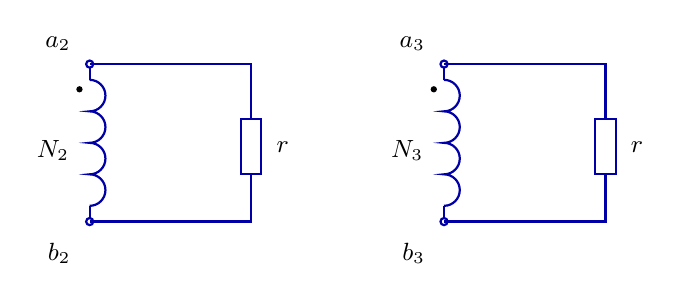
\begin{tikzpicture}[font=\small]
\begin{scope}
\coil{0}{2}{}
\draw[wire](0,2.8)--(2.05,2.8)--(2.05,2.10);
\draw[wire](2.05,2.10)++(-.13,0)rectangle++(.26,-.70);
\draw[wire](2.05,1.40)--(2.05,.8)--(0,.8);
\node[right]at(2.25,1.75){$r$};
\end{scope}
\begin{scope}[xshift=4.5cm]
\coil{0}{3}{}
\draw[wire](0,2.8)--(2.05,2.8)--(2.05,2.10);
\draw[wire](2.05,2.10)++(-.13,0)rectangle++(.26,-.70);
\draw[wire](2.05,1.40)--(2.05,.8)--(0,.8);
\node[right]at(2.25,1.75){$r$};
\end{scope}
\end{tikzpicture}
\begin{tikzpicture}[font=\small]
\begin{scope}
\coil{0}{2}{}\coil{3}{3}{}
\draw[wire](0,.8)--(1.30,.8)--(1.30,3.55)--(3,3.55)--(3,2.8);
\draw[wire](0,2.8)--(-1.05,2.8)--(-1.05,-.55)--(-.25,-.55);
\resistorH{-.25}{-.55}{r}
\draw[wire](.80,-.55)--(1.95,-.55);\resistorH{1.95}{-.55}{r}
\draw[wire](3,-.55)--(4.10,-.55)--(4.10,.8)--(3,.8);
\node[above]at(1.5,4.15){串联相助};
\end{scope}
\begin{scope}[xshift=7.0cm]
\coil{0}{2}{}\coil{3}{3}{}
\draw[wire](0,.8)--(0,.20)--(3,.20)--(3,.8);
\draw[wire](0,2.8)--(-1.05,2.8)--(-1.05,3.55)--(-.25,3.55);
\resistorH{-.25}{3.55}{r}
\draw[wire](.80,3.55)--(1.95,3.55);\resistorH{1.95}{3.55}{r}
\draw[wire](3,3.55)--(4.10,3.55)--(4.10,2.8)--(3,2.8);
\node[above]at(1.5,4.15){串联相消};
\end{scope}
\end{tikzpicture}
\begin{tikzpicture}[font=\small]
\begin{scope}
\draw[gray](0,0)--(2.6,0)(0,1.4)--(2.6,1.4)(0,4)--(2.6,4);
\node[left]at(0,0){$b_3$};\node[left]at(0,1.4){$b_2=a_3$};\node[left]at(0,4){$a_2$};
\node[right]at(2.6,0){$0$};\node[right]at(2.6,1.4){$u_3$};\node[right]at(2.6,4){$u_2+u_3$};
\draw[blue!65!black,thick,->](.6,0)--(.6,1.4)node[midway,right]{$u_3$};
\draw[blue!65!black,thick,->](.6,1.4)--(.6,4)node[midway,right]{$u_2$};
\draw[orange!85!black,thick,<->](2,0)--(2,4);
\node[above]at(1.1,4.5){相助};
\end{scope}
\begin{scope}[xshift=6.4cm]
\draw[gray](0,0)--(2.6,0)(0,1.4)--(2.6,1.4)(0,2.6)--(2.6,2.6);
\node[left]at(0,0){$b_2=b_3$};\node[left]at(0,1.4){$a_3$};\node[left]at(0,2.6){$a_2$};
\node[right]at(2.6,0){$0$};\node[right]at(2.6,1.4){$u_3$};\node[right]at(2.6,2.6){$u_2$};
\draw[blue!65!black,thick,->](.6,0)--(.6,1.4)node[midway,right]{$u_3$};
\draw[blue!65!black,thick,->](1.3,0)--(1.3,2.6)node[pos=.80,left]{$u_2$};
\draw[orange!85!black,thick,<->](2,1.4)--(2,2.6);
\node[above]at(1.1,4.5){相消};
\end{scope}
\node[below]at(4.2,-.45){示意取$u_2>u_3>0$；橙色线段为负载电压跨度};
\end{tikzpicture}
\end{document}
